\section{Example}\label{chap:kokkosExample}

In order to provide an impression of the looks and feel of Kokkos code this section discusses a small but complete example of a data parallel Kokkos application shown in Figure~\ref{fig:KokkosExample} which allocates data, potentially initalizes it on the host and then performs a matrix-vector product.
Similar to other programming models such as MPI, Kokkos must be initialized and finalized. 
This serves the purpose of setting up the underlying runtime and acquiring resouces.
The fundamental data structure of Kokkos programs is the ~\emph{Kokkos::View}.
These views represent multi-dimensional arrays of rank one to eight.
A general philosophy of Kokkos is to have defaults for most properties, including data layouts, memory spaces and execution spaces.
Consequently the simple example does not explicitly set which memory space the data lives in.
Kokkos ensures that the defaults for parallel execution and data allocations match though. 

The example then creates copies of the views accessible by the host process via the ~\emph{create\_mirror\_view} function. 
If the original data was already accessible by the host process, this function returns a ~\emph{View} referencing the same allocation.
In real applications this host process accessible allocation is often necessary for I/O purposes for example to initialize the data with input read from a file.
To get the data to the memory space accessible by the parallel execution resources the function ~\emph{deep\_copy} is then invoked.
If two ~\emph{View}s are aliases of each other this operation is a no-op. 

Now the parallel pattern can be invoked.
Since the matrix-vector product is an example of hierarchical work (for each row a dot product must be performed), the ~\emph{Kokkos::TeamPolicy} is used.
For each row of M a team of threads is launched, where the size of team is left for the Kokkos runtime to choose.
When using a ~\emph{TeamPolicy} the operator of the lambda does not simply get an index, but rather a handle to the team of threads. 
This handle provides the team id, and is subsequently handed to the nested parallel execution policies. 
The nested reduction requires the operator of the nested lambda to take a reference to the thread local reduction variable (called here ~\emph{y\_tmp}) in addition to the loop index.
It then writes the result into the correct position of the output vector. 

After the parallel pattern the main code calls a fence to ensure that the execution of the parallel code is finished, before copying the results of y back to the host and potentially putting them out through an I/O operation.

To learn more about Kokkos's capabilties and features we recommend going through the extensive Kokkos tutorial, with multiple days worth of lectures and exercises, and read the Kokkos Programming Guide as well as the Kokkos API documentation - which provide several hundred pages of text-book like material and API reference.
The Tutorial is intended for computational scientists with minimal or even no prior knowlegde of parallel programming.
It introduces concepts of parallel programming using Kokkos step by step, through a series of lectures and hands-on exercises which build on each other and gradually introduce more and more Kokkos constructs.
The Programming Guide provides more in-depth information to the concepts introduced in the Tutorial, while the API reference provides straight forward documentation of the syntax and semantics of Kokkos's library interface.

\begin{figure}
\begin{small}
\begin{Verbatim}[frame=leftline]
#include<Kokkos_Core.hpp>
int main(int argc, char* argv[]) {
  Kokkos::initialize(argc,argv);
  {
    Kokkos::View<double*> x("x", M);  
    Kokkos::View<double*> y("y", N);
    Kokkos::View<double**,Kokkos::LayoutRight> A("A", N, M);  

    auto x_h = Kokkos::create_mirror_view(x);
    auto y_h = Kokkos::create_mirror_view(y);
    auto A_h = Kokkos::create_mirror_view(A);
    //intialize_data_on_host(x_h,A_h);
    Kokkos::deep_copy(x,x_h);
    Kokkos::deep_copy(A,A_h);    

    Kokkos::parallel_for("outer", TeamPolicy<>(N,AUTO),
    [=](const member_type &team_handle) {
      const int e = team_handle.league_rank();
      Kokkos::parallel_reduce( TeamThreadRange(team_handle, M),
        [=](const int & i, double & y_tmp) {
          y_tmp += A(e, i) * x(i);
        }, 
        y(e));
    }); 
    Kokkos::fence();
    Kokkos::deep_copy(y_h,y);
    //output_result_on_host(y_h);
  }
  Kokkos::finalize();
}
\end{Verbatim}
\end{small}
\caption{This example application written in Kokkos shows the use of a~\emph{view}-type and a parallel for loop using a ~\emph{TeamPolicy} and a nested parallel reduction. }
\label{fig:KokkosExample}
\end{figure}


\section{Kokkos Implementation}

The following section gives a short impression of Kokkos maps generic parallel programming patterns to the hardware specific programming models.
As a template metaprogramming library, Kokkos makes heavy use of partial specialization. 
In particular the parallel pattern functions are mapped to partial specializations of classes for those patterns for each execution policy type and backend type.
The library specification contains concepts for execution spaces, which define the generic interface of those classes.
To add a new backend, each of those concepts must be implemented.

A simplified version of this implementation strategy is provided in Figure\ref{fig:KokkosExampleOMPBackEnd}.
The ~\emph{parallel\_for} function instantiates a partial specialization of the ~\emph{ParallelFor} class and calls its ~\emph{execute} function.
That function is then responsible to implement the Kokkos parallel pattern, for example via OpenMP pragmas in the case of the OpenMP execution space.
\begin{figure}
\begin{small}
\begin{Verbatim}[frame=leftline]
template <class FunctorType>
class ParallelFor<FunctorType, RangePolicy<OpenMP> > {
  const FunctorType functor;
  const RangePolicy<OpenMP> policy; 

public:
  void execute() const {
    #pragma omp parallel for
    for(int i=policy.begin(); i<policy.end(); i++)
      functor(i);
  }
}

template <class FunctorType, class PolicyType>
void parallel_for(std::string label, const PolicyType& policy,
                  const FunctorType& functor) {
  // Call tools hook with label
  ParallelFor<FunctorType,PolicyType> pf{functor,policy};
  pf.execute();
}

\end{Verbatim}
\end{small}
\caption{This code shows the back-end implementation of a parallel loop in the Kokkos programing model. It shows a particular implementation of that generic pattern as a templated class to the OpenMP execution space. Also it shows the use of OpenMP pragma annotations that put platform compilers in charge to generate parallel code for the underlying hardware architecture.}
\label{fig:KokkosExampleOMPBackEnd}
\end{figure}


%\begin{figure}
%\centerline{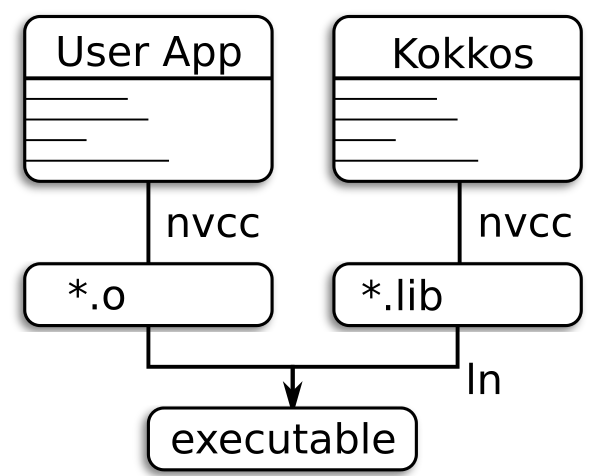
\includegraphics[width=0.3\textwidth]{img/Build.png}}
%\caption{The compilation workflow includes the invocation of the platform compiler that is in charge to generate parallel   Building workflow}
%\label{fig:workflow}  
%\end{figure}
